\documentclass{sciposter}
\usepackage[utf8]{inputenc}
\usepackage[brazil]{babel}
\usepackage{multicol}
\usepackage{amsmath, amssymb}
\usepackage{graphicx}
\usepackage{tabularx}
\usepackage{multirow}
\usepackage{booktabs}
\usepackage{textcomp} % for registred symbol
\usepackage[linesnumbered,algoruled,longend]{algorithm2e}

\newcommand{\midsepremove}{\aboverulesep = 0mm \belowrulesep = 0mm}
\midsepremove
\newcommand{\midsepdefault}{\aboverulesep = 0.605mm \belowrulesep = 0.984mm}
\midsepdefault

\title{Vulnerability Detection via Topological Analysis of Attention Maps}

\author{P. Snopov, A. N. Golubinsky}

\institute 
{IITP RAS}

\email{snopov@iitp.com}

\leftlogo[1.35]{img/iitp.png}
\rightlogo[0.7]{img/itas.png}

%%%%%%%%%%%%%%%%%%%%%%%%%%%%%%%%%%%%%%%%%%%%%%%%%%%%%%%%%%%%%%%%%%%%%%%%%%%%%%%%
%%% Begin of Document

\begin{document}


\conference{The 48th ITaS School and Conference: Information Technologies and Systems}

\maketitle

\newcommand{\mycaption}{%
\ifx \@captype \@undefined \@latex@error {\noexpand \caption outside float}\@ehd \expandafter \@gobble \else \refstepcounter \@captype \expandafter \@firstofone \fi {\@dblarg {\@caption \@captype }}%
}%

%%% Begin of Multicols-Enviroment
\begin{multicols}{3}

%%% Abstract
% \begin{abstract}
% Abstract.
% \end{abstract}

%%% Introduction
\section{Introduction}


The problem of source code vulnerability detection has become increasingly 
important in the field of software engineering. This complex task involves analyzing 
both the syntax and semantics of the source code. Traditionally, static analysis 
methods have dominated the field of vulnerability detection. 
These static tools tend to rely heavily on the syntax of the program, thereby 
overlooking potential information hidden in the semantics. As a result, 
such approaches often suffer from high rates of false positives.

Our work presents a novel approach to the vulnerability detection problem.
As previously mentioned, the superiority of DL-based models over static ones is 
potentially due to their ability to capture the semantic information of the program. 
This semantic information is captured by the neural networks during training or 
fine-tuning. Furthermore, LLM-based models can capture this information even without 
fine-tuning.

In this work, we leverage the BERT model, pre-trained on source code, to capture the 
semantic information of programs. We also utilize tools from topological 
data analysis to explore the relationships within this semantic 
information. Our aim is to analyze and interpret the attention matrices using 
topological instruments.

Our work is inspired by the work of Laida Kushareva et. al., 
in which the authors apply the topological methods for the artificial text detection. They demonstrated that 
the topology of the semantics captured by an LLM model (such as BERT) provides 
sufficient information for successful classification. Their approach outperformed 
neural baselines and performed on par with a fully fine-tuned BERT model, while being 
more robust to unseen data.

\section{Theoretical background}

Topological data analysis (TDA) is an emerging field that applies algebraic topology methods to data science. The main tool in topological data analysis, {\bf persistent homology},  tracks changes in the topological structure of various objects, such as point clouds, scalar functions, images, and weighted graphs.

An {\bf attention graph} is a weighted graph representation of an attention matrix $W^{attn}$, 
where vertices represent the tokens and the edges connect a pair of tokens if the 
corresponding weight exceeds a predefined threshold value.

In our work, given a set of tokens $V$ and an attention matrix $W$,we construct a 
family of attention graphs indexed by increasing threshold values. This family, known 
as a {\bf filtration}, is a fundamental object in TDA.

With this sequence of graphs, we compute persistent homology in dimensions $0$ and $1$.
Dimension $0$ reveals connected components or clusters in the data, while 
dimension $1$ identifies cycles or "loops". 
These computations yield a {\bf persistence diagram}, which can be used to derive 
specific topological features, such as the number of connected components and 
cycles (such features are also called the {\it Betti numbers}).

\begin{figure}
  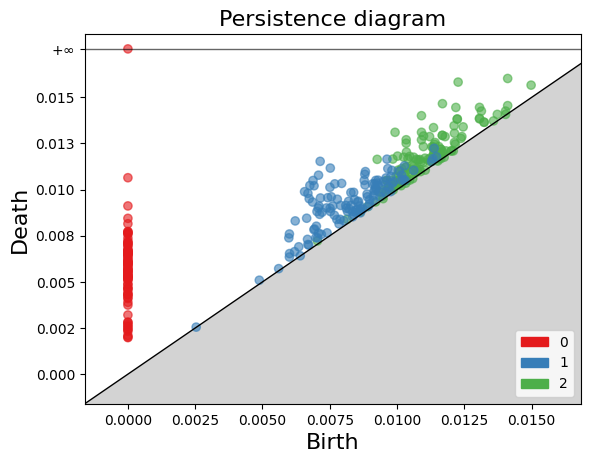
\includegraphics{img/pd}
  \centering
  \caption{Example of a PD of some attention matrix}
\end{figure}


\section{Topological Features of the Attention Graphs}

For each code sample, we calculate the persistent homology in dimensions $0$ and $1$ of 
the symmetrized attention matrices, obtaining the persistence diagram for each 
attention head of the BERT model. We compute the following features in each dimension 
from the diagrams:
\begin{itemize}
    \item Mean lifespan of points on the diagram
    \item Variance of the lifespan of points on the diagram
    \item Maximum lifespan of points on the diagram
    \item Total number of points on the diagram
    \item Persistence entropy
\end{itemize}

We symmetrize attention matrices to enable the application of persistent homology techniques. 
Symmetrizing attention matrices allows us to interpret them as distance matrices of a point cloud embedded in Euclidean space. 
We symmetrize attention matrices as follows: 
\begin{equation}
    \forall i,j: W^\mathrm{sym}_{ij} = \max{(W_{ij}^\mathrm{attn}, W_{ji}^\mathrm{attn})}.
\end{equation}

Alternatively, one can think of attention graphs, in which an edge between the vertices $i$ and $j$
appears if the threshold is greater than both $W_{ij}^\mathrm{attn}$ and $W_{ji}^\mathrm{attn}$.

We consider these features as the numerical characteristics of the semantic evolution processes 
in the attention heads. These features encode the information about the clusters of mutual influence
of the tokens in the sentence and the local structures like cycles. The features with "significant"\space 
persistence (i.e. those with large lifespan) correspond to the stable processes, whileas the features
with short lifespans are highly susceptible to noise and do not reflect the stable topological attributes.

\section{Experiments}
\subsection*{Methodology} 
To evaluate whether the encoded topological information can be used for 
vulnerability detection, we train Logistic Regression, Support Vector Machine (SVM), 
and Gradient Boosting classifiers on the topological features derived from the 
attention matrices of the BERT model. 

We utilize the {\it scikit-learn} library for Logistic Regression 
and SVM, and the {\it LightGBM} library for Gradient Boosting.

\subsection*{Data} 
We train and evaluate our classifier on {\it Devign} dataset.
This dataset comprises samples from two large, widely-used open-source C-language projects: QEMU, and FFmpeg, 
which are popular among developers and diverse in functionality.
Due to computational constraints, we were only using those data samples, that, 
being tokenized, are of length less than $150$. This ensures that the point cloud 
constructed during attention symmetrization is also limited to a maximum length of $150$.

\subsection*{Baselines} 
We employ the \texttt{microsoft/codebert-base} model from the 
HuggingFace library as our pre-trained BERT-based baseline. 
Additionally, we fully fine-tune the \texttt{microsoft/codebert-base} model for comparison.

\section{Results and Discussion}

\begin{table}
    \label{tab:results}
    \centering
    \caption{The results of the vulnerability detection experiments.}\label{results}
    \begin{tabular}{|c|c|c|}
    \hline
    {\bf Model} & {\bf F1 score} & {\bf Accuracy} \\
    \hline
    Logistic Regression & 0.22 & 0.54 \\
    \hline
    LightGBM & {\bf 0.55} & 0.63 \\
    \hline
    SVM & 0.54 & {\bf 0.65} \\
    \hline
    CodeBERTa (pre-trained) & 0.28 & 0.45 \\
    \hline
    CodeBERTa (fine-tuned) & {\bf 0.71} & {\bf 0.72} \\
    \hline
    \end{tabular}
\end{table}

The table outlines the results of the vulnerability detection experiments 
on the {\it Devign} dataset. The results reveal that the proposed topology-based 
classifiers outperform the chosen LLM without fine-tuning but perform worse than the fine-tuned version.
  
\section{Acknowledgements}
The work was carried out as part of the state assignment N 1021061609772-0-1.2.1
(FFNU-2024-0020).

\end{multicols}

\end{document}
